\chapter{CI/CD}
\label{ch:cicd}

\section{Overview}

\textbf{Status:} PARTIAL.

The repository contains two GitHub Actions workflows in
\texttt{.github/workflows/}. There is no CI workflow in the conventional sense:
nothing runs on pull requests or pushes to validate the code. Both workflows are
\emph{delivery} workflows triggered by merge or tag.

\begin{figure}[H]
\centering
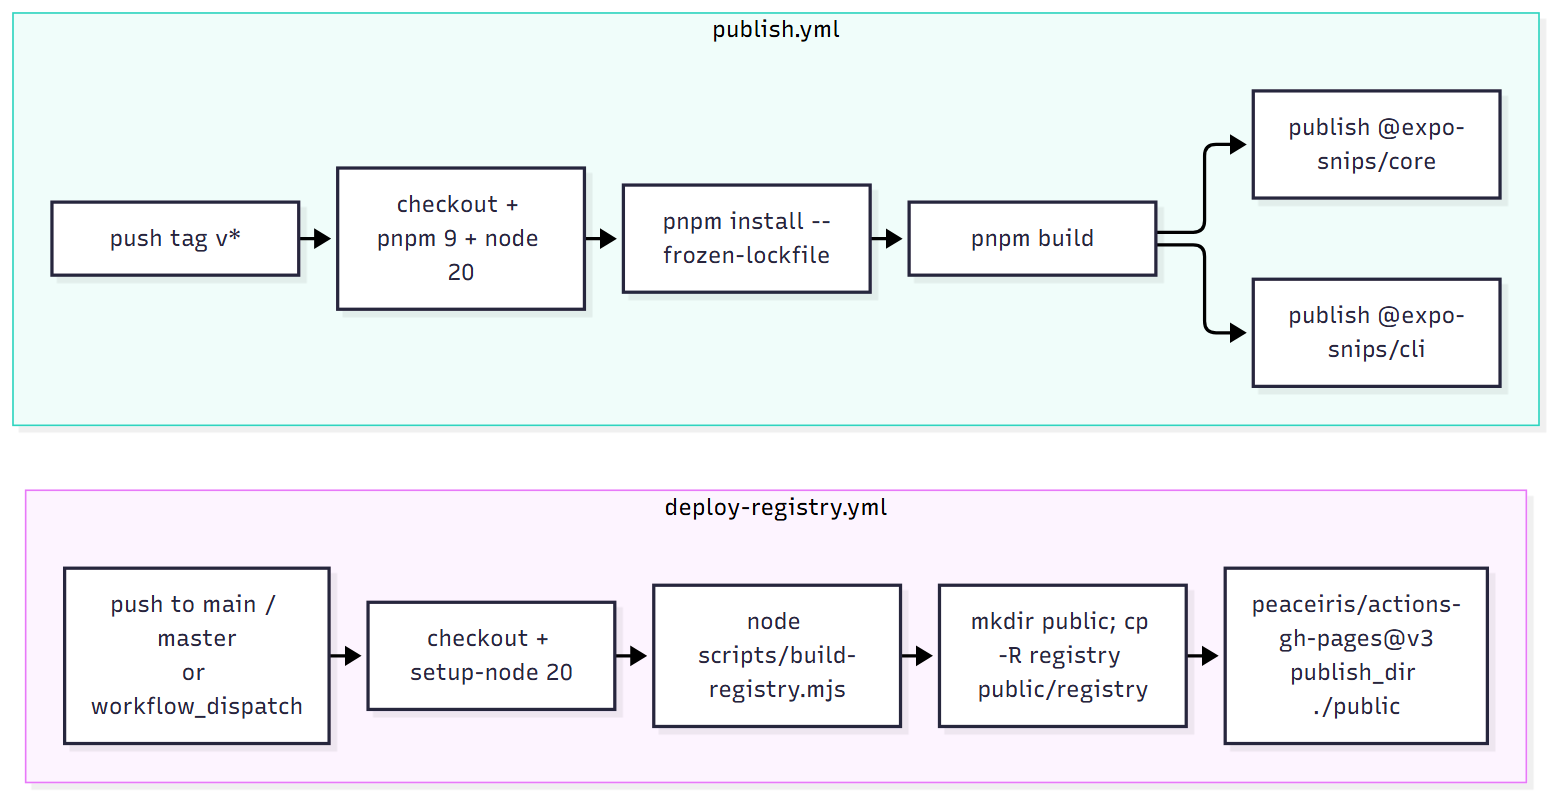
\includegraphics[width=\textwidth]{diagrams/cicd-deployment.png}
\caption{Continuous delivery pipelines present in the repository}
\label{fig:cicd-deployment}
\end{figure}

\section{Workflow inventory}

\begin{longtable}{@{}L{3.2cm}L{3.4cm}L{3.4cm}L{4.2cm}@{}}
\caption{GitHub Actions workflows}\\
\toprule
\textbf{File} & \textbf{Trigger} & \textbf{Runner} & \textbf{Purpose} \\
\midrule
\endfirsthead
\toprule
\textbf{File} & \textbf{Trigger} & \textbf{Runner} & \textbf{Purpose} \\
\midrule
\endhead
\texttt{publish.yml} & push to tags \texttt{v*} & ubuntu-latest, Node 20,
pnpm 9 & Build all packages and publish \texttt{@expo-snips/core} and
\texttt{@expo-snips/cli} to npm. \\
\texttt{deploy-registry.yml} & push to \texttt{main}/\texttt{master},
\texttt{workflow\_dispatch} & ubuntu-latest, Node 20 & Build the registry and
deploy it to GitHub Pages. \\
\bottomrule
\end{longtable}

\section{Pipeline detail: \texttt{publish.yml}}

\begin{enumerate}
  \item \texttt{actions/checkout@v4}
  \item \texttt{pnpm/action-setup@v4} (version 9)
  \item \texttt{actions/setup-node@v4} (Node 20, \texttt{registry-url:
        https://registry.npmjs.org})
  \item \texttt{pnpm install --frozen-lockfile} --- reproducible install from the
        committed lockfile.
  \item \texttt{pnpm build} --- recursive build; this runs
        \texttt{prepare-registry.mjs} for both clients before compilation.
  \item Publish \texttt{core}, then publish \texttt{cli}, each authenticated with
        \texttt{NPM\_TOKEN}.
\end{enumerate}

Notes: publishing uses \texttt{--no-git-checks} (permitting a publish from a
detached HEAD, which is normal on a tag build) and \texttt{--access public}
(reinforcing the package's own \texttt{publishConfig}). There is no headless
\texttt{npm whoami} check, no provenance/attestation step, and no dry-run gate.

\section{Pipeline detail: \texttt{deploy-registry.yml}}

\begin{enumerate}
  \item \texttt{actions/checkout@v4}
  \item \texttt{actions/setup-node@v4} (Node 20; no dependency install step
        because the script uses only Node built-ins)
  \item \texttt{node scripts/build-registry.mjs} --- rebuilds
        \texttt{registry/}
  \item \texttt{mkdir public} and \texttt{cp -R registry public/registry}
  \item \texttt{peaceiris/actions-gh-pages@v3} publishes \texttt{./public} to
        \texttt{gh-pages} using \texttt{GITHUB\_TOKEN}, under
        \texttt{contents: write} permission.
\end{enumerate}

\section{What the pipelines do not do}

\begin{longtable}{@{}L{4.6cm}L{2.2cm}L{7.4cm}@{}}
\caption{Missing pipeline capabilities}\\
\toprule
\textbf{Capability} & \textbf{Present?} & \textbf{Comment} \\
\midrule
\endfirsthead
\toprule
\textbf{Capability} & \textbf{Present?} & \textbf{Comment} \\
\midrule
\endhead
Linting & No & No linter is configured anywhere in the repo. \\
Automated tests & No & No tests exist; no test step is present. \\
Recipe validation in CI & No & \texttt{validate.mjs} exists but is not invoked by
either workflow. \\
Build on pull requests & No & Neither workflow runs on \texttt{pull\_request}. \\
Type checking & Indirect & \texttt{pnpm build} runs \texttt{tsc}, so type errors
fail the delivery build --- but only after merge or on a tag, not on a PR. \\
Dependency audit & No & No \texttt{pnpm audit}, Dependabot or CodeQL. \\
Extension packaging/publish & No & The VSIX is built and committed by hand. \\
Caching & No & No \texttt{actions/cache} or pnpm store cache configured. \\
Provenance / attestation & No & Plain \texttt{npm publish}. \\
Version bumping & No & Version numbers are edited manually in
\texttt{package.json}. \\
\bottomrule
\end{longtable}

\section{Consequences}

\begin{itemize}
  \item \textbf{The pipeline cannot prevent a broken main.} Because no workflow
        runs on pull requests, a change that fails to build or violates the
        recipe schema is only discovered when someone builds locally --- or when
        a tag is pushed and publishing fails.
  \item \textbf{The registry is rebuilt on every push to the default branch.}
        This is good for freshness but means an unreviewed change to a template
        reaches the published registry immediately after merge.
  \item \textbf{The extension lags the rest of the product.} The CLI and registry
        are automated while the extension, the most user-facing artefact, is
        manual.
  \item \textbf{No concurrency control on \texttt{deploy-registry.yml}.} Two rapid
        pushes could race to push the \texttt{gh-pages} branch; there is no
        \texttt{concurrency} group.
\end{itemize}

\section{Recommended pipeline}

\textbf{Status:} RECOMMENDED. A minimal, high-value CI workflow on
\texttt{pull\_request} and \texttt{push} to the default branch would:

\begin{enumerate}
  \item check out, install with \texttt{--frozen-lockfile};
  \item run \texttt{node scripts/validate.mjs} (recipe integrity);
  \item run \texttt{pnpm build} (type-check and compile all packages);
  \item run tests once they exist (see Chapter~\ref{ch:testing});
  \item add a linter and formatter check;
  \item enable dependency update automation.
\end{enumerate}

Then add a \texttt{concurrency} group to the registry deployment workflow and a
tag-triggered job that packages the extension.

\section{CI/CD summary}

\begin{table}[H]
\centering
\caption{CI/CD posture}
\begin{tabular}{@{}L{4cm}L{10.2cm}@{}}
\toprule
\textbf{Dimension} & \textbf{Assessment} \\
\midrule
Continuous integration & NOT IMPLEMENTED (no PR validation). \\
Continuous delivery --- npm & IMPLEMENTED (tag-triggered). \\
Continuous delivery --- registry & IMPLEMENTED (push-triggered). \\
Continuous delivery --- extension & NOT IMPLEMENTED (manual). \\
Quality gates in CI & None beyond compilation. \\
\bottomrule
\end{tabular}
\end{table}
